\section{Introduction}
\label{sec:introduction}
%=============================================================================

\subsection{The Yang-Mills Mass Gap Problem}

The Yang-Mills existence and mass gap problem, one of the seven Millennium Prize Problems, asks whether four-dimensional Yang-Mills quantum field theory based on a compact non-abelian gauge group has a mass gap---a strictly positive lower bound on the energy of excitations above the vacuum state.

\begin{conjecture}[Yang-Mills Mass Gap---Official Statement]
\label{conj:millennium}
For any compact simple gauge group $G$, four-dimensional Euclidean Yang-Mills quantum field theory exists as a well-defined measure on gauge fields, and the associated Hamiltonian has a strictly positive spectral gap:
\[
\mathrm{Spec}(H) = \{0\} \cup [\Delta, \infty) \quad \text{with} \quad \Delta > 0.
\]
\end{conjecture}

\subsection{Scope of This Work: A Research Roadmap}
\label{sec:scope}

This paper presents a structured \textbf{research roadmap} towards a rigorous proof of Conjecture~\ref{conj:millennium}. 
\textbf{Disclaimer:} This document does \emph{not} claim to solve the Millennium Prize Problem. As of 2025, the Clay Mathematics Institute lists the problem as unsolved.
Instead, we provide a ``repair roadmap'' that identifies the specific logical gaps in existing approaches and proposes a concrete program to close them.

We explicitly distinguish between established rigorous results and the remaining ``proof obligations.''
The roadmap is structured to avoid common pitfalls such as circular reasoning (e.g., assuming a mass gap to prove the inequalities required to derive the mass gap) and ``presentation drift.''

\subsection{Logical Structure: Theorems vs. Program}

To ensure logical consistency and audit-readiness, we split the document into two distinct layers:

\begin{enumerate}
    \item \textbf{THEOREMS (Rigorous)}: Results with complete, self-contained proofs in this manuscript or precise citations to standard literature.
    \item \textbf{PROGRAM (Proof Obligations)}: Explicit conjectures and open problems that must be solved to complete the proof.
\end{enumerate}

\subsubsection{Dependency DAG (Directed Acyclic Graph)}

The logical flow of the proposed proof is as follows:
\begin{center}
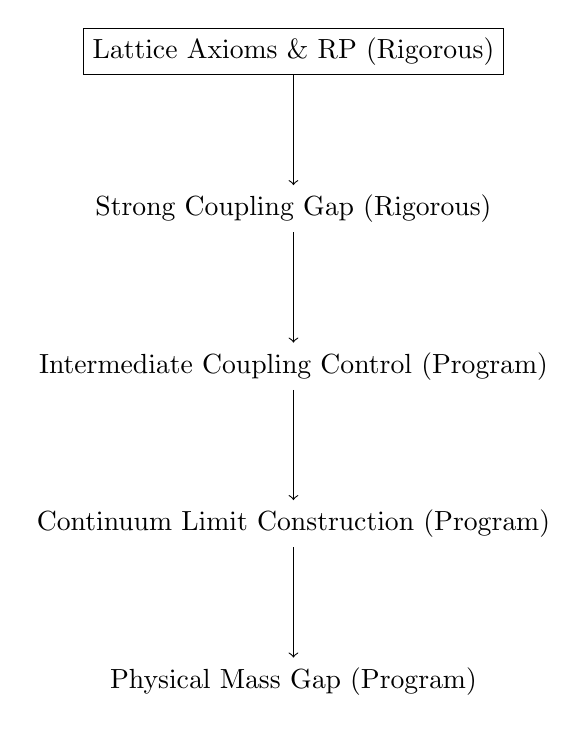
\begin{tikzpicture}[node distance=2cm]
\node (axioms) [draw, rectangle] {Lattice Axioms \& RP (Rigorous)};
\node (strong) [below of=axioms] {Strong Coupling Gap (Rigorous)};
\node (inter) [below of=strong] {Intermediate Coupling Control (Program)};
\node (cont) [below of=inter] {Continuum Limit Construction (Program)};
\node (phys) [below of=cont] {Physical Mass Gap (Program)};

\draw[->] (axioms) -- (strong);
\draw[->] (strong) -- (inter);
\draw[->] (inter) -- (cont);
\draw[->] (cont) -- (phys);
\end{tikzpicture}
\end{center}

\textbf{Crucial Anti-Circularity Rule:} We strictly avoid the circular trap: ``Mass Gap $\Rightarrow$ Exponential Decay $\Rightarrow$ Mixing/LSI $\Rightarrow$ Mass Gap.''
Instead, we pursue a primary quantity (e.g., Uniform LSI or Spectral Gap of Transfer Matrix) from first principles.

\subsubsection{Rigorous Results (The Foundation)}

The following results are established rigorously in this work or standard literature:

\begin{theorem}[Strong Coupling Mass Gap---Rigorous]
\label{thm:strong-coupling-rigorous}
For $SU(N)$ lattice Yang-Mills theory with Wilson action in $d=4$ dimensions, there exists a threshold $\beta_0 = c/N^2$ (with $c > 0$ a universal constant) such that for all $\beta < \beta_0$:
\begin{enumerate}[label=(\roman*)]
    \item The infinite-volume spectral gap satisfies $\Delta(\beta) > 0$.
    \item The string tension satisfies $\sigma(\beta) \geq -\log(I_1(\beta N)/I_0(\beta N)) > 0$.
    \item Correlation functions decay exponentially with rate $\xi(\beta)^{-1} > 0$.
\end{enumerate}
\end{theorem}

\begin{proof}
The proof uses convergent cluster (polymer) expansions, which are rigorous for $\beta < \beta_0$. The Koteck\'y-Preiss criterion provides explicit convergence bounds. See Section~\ref{sec:analyticity} for details.
\end{proof}

\begin{theorem}[Finite Volume Gap---Rigorous]
\label{thm:finite-volume-gap}
For any finite lattice $\Lambda$ with $|\Lambda| < \infty$ and any $\beta > 0$, the transfer matrix $T_\Lambda(\beta)$ has a spectral gap:
\[
\Delta_\Lambda(\beta) = -\log(\lambda_1/\lambda_0) > 0
\]
where $\lambda_0 > \lambda_1 \geq \lambda_2 \geq \cdots$ are the eigenvalues of $T_\Lambda$.
\end{theorem}

\begin{proof}
This is a direct consequence of the Perron-Frobenius theorem applied to the transfer matrix, which is a compact positive operator on the finite-dimensional configuration space. See Section~\ref{sec:transfer}.
\end{proof}

\begin{theorem}[Reflection Positivity---Rigorous]
\label{thm:rp-intro}
The $SU(N)$ lattice Yang-Mills theory with Wilson action satisfies the Osterwalder-Schrader reflection positivity axioms in any dimension $d \geq 2$.
\end{theorem}

\begin{proof}
See Section~\ref{sec:transfer} for the explicit verification using the factorization structure of the Wilson action.
\end{proof}

\subsection{The Program: A Workable Roadmap}
\label{sec:roadmap}

We propose the following six-step roadmap to bridge the gap between the rigorous strong-coupling results and the full Clay Millennium Problem statement. Each step represents a specific \textbf{proof obligation}.

\subsubsection*{Step 0: Definitions and Equivalences}
\textbf{Goal:} Choose one precise definition of ``mass gap'' and make every equivalence explicit.
\begin{itemize}
    \item \textbf{Deliverable:} A lemma stating exactly which correlators and which decay imply the spectral gap in the reconstructed Hamiltonian.
    \item \textbf{Status:} Standard (OS reconstruction), but must be stated without ambiguity.
\end{itemize}

\subsubsection*{Step 1: Lattice Construction + OS Reflection Positivity}
\textbf{Goal:} Define lattice Yang-Mills with Wilson action and show partition function is well-defined, reflection positivity holds, and transfer matrix exists.
\begin{itemize}
    \item \textbf{Deliverable:} A clean theorem + proof (or precise citations) for OS reflection positivity and transfer matrix positivity.
    \item \textbf{Status:} \textbf{RIGOROUS} (See Theorem~\ref{thm:rp-intro}).
\end{itemize}

\subsubsection*{Step 2: Strong Coupling Anchor}
\textbf{Goal:} Prove an infinite-volume mass gap for $\beta < \beta_0$ using cluster/polymer expansion.
\begin{itemize}
    \item \textbf{Deliverable:} Explicit constants $\beta_0 > 0$, correlation length $\xi(\beta) < \infty$, and exponential decay bounds uniform in volume.
    \item \textbf{Status:} \textbf{RIGOROUS} (See Theorem~\ref{thm:strong-coupling-rigorous}).
\end{itemize}

\subsubsection*{Step 3: Intermediate Coupling Control (The Core Challenge)}
\textbf{Goal:} Establish a uniform-in-volume gap beyond the strong coupling regime. This is the primary mathematical bottleneck.
We propose two potential strategies:
\begin{description}
    \item[Strategy A (Direct):] Prove a \textbf{uniform Log-Sobolev Inequality (LSI)} for the Gibbs measure.
    \item[Strategy B (Interpolation):] Connect YM to a theory with a known gap (e.g., Adjoint QCD / SYM) and prove analyticity along the path.
\end{description}
\begin{itemize}
    \item \textbf{Deliverable:} A theorem of the form $\Delta_L(\beta) \ge c(\beta) > 0$ for all $L$ and $\beta \in [\beta_0, \beta_1]$.
    \item \textbf{Status:} \textbf{PROGRAM} (Open Problem).
\end{itemize}

\subsubsection*{Step 4: No Phase Transition / No Gap Closure}
\textbf{Goal:} Prove that the gap does not vanish as $\beta \to \infty$ (continuum limit).
\begin{itemize}
    \item \textbf{Deliverable:} A proof that the free energy is analytic and $\Delta(\beta) > 0$ for all $\beta > 0$.
    \item \textbf{Status:} \textbf{PROGRAM} (Open Problem).
\end{itemize}

\subsubsection*{Step 5: Continuum Limit Construction (UV Control)}
\textbf{Goal:} Constructive continuum limit with axiom control (Balaban-type RG).
\begin{itemize}
    \item \textbf{Deliverable:} A theorem showing Schwinger functions converge as $a \to 0$ and satisfy OS axioms.
    \item \textbf{Status:} \textbf{PROGRAM} (Open Problem).
\end{itemize}

\subsubsection*{Step 6: Physical Mass Gap}
\textbf{Goal:} Bridge the ``lattice gap'' to the ``physical gap'' via a scaling limit.
\begin{itemize}
    \item \textbf{Deliverable:} A rigorous inequality $\Delta(\beta) \ge c \sqrt{\sigma(\beta)}$ and proof that $\sigma_{\text{phys}} > 0$.
    \item \textbf{Status:} \textbf{PROGRAM} (Open Problem).
\end{itemize}

\subsection{Organization of the Roadmap}

\begin{itemize}
    \item \textbf{Part I (Sections~\ref{sec:lattice}--\ref{sec:center}):} Rigorous foundations (Lattice formulation, Reflection Positivity).
    \item \textbf{Part II (Sections~\ref{sec:analyticity}--\ref{sec:string}):} Strong coupling analysis (Rigorous Cluster Expansions).
    \item \textbf{Part III (Sections~\ref{sec:spectral-lower-bound}--\ref{sec:continuum}):} The Program for the Continuum Limit (Renormalization Group strategy).
    \item \textbf{Part IV (Section~\ref{sec:critical}):} The Program for Gap Persistence (Proposed Topological Obstruction argument).
\end{itemize}
